\documentclass[conference]{IEEEtran}
\IEEEoverridecommandlockouts
% The preceding line is only needed to identify funding in the first footnote. If that is unneeded, please comment it out.
\usepackage{cite}
\usepackage{amsmath,amssymb,amsfonts}
\usepackage{algorithmic}
\usepackage{graphicx}
\usepackage{textcomp}
\usepackage{xcolor}
\usepackage{array}
\usepackage{listings}
\def\BibTeX{{\rm B\kern-.05em{\sc i\kern-.025em b}\kern-.08em
    T\kern-.1667em\lower.7ex\hbox{E}\kern-.125emX}}

\sloppy

\begin{document}

\title{On a Deep Q-Network-based Approach \\
for Active Queue Management}

\author{
\IEEEauthorblockN{
Dhulfiqar A. AlWahab\IEEEauthorrefmark{1}\IEEEauthorrefmark{2},
Gerg\H{o} Gombos\IEEEauthorrefmark{2},
S\'andor Laki\IEEEauthorrefmark{2}
}
\IEEEauthorblockA{
\IEEEauthorrefmark{1}3in Research Group, ELTE E\"{o}tv\"{o}s Lor\'and University, Martonv\'as\'ar, Hungary\\
\IEEEauthorrefmark{2}Communication Networks Laboratory, ELTE E\"{o}tv\"{o}s Lor\'and University, Budapest, Hungary\\ \{aalwahab, ggombos, lakis\}@inf.elte.hu}
}

\maketitle

\begin{abstract}
Reinforcement learning has gone through an enormous evolution in the past ten years. It's practical applicability has been demonstrated through several use cases in various fields from robotics to process automation. In this paper, we examine how the tools of deep Q-learning can be used in an AQM algorithm to reduce queuing delay and ensure good link utilization at the same time. The proposed method called RL-AQM has the advantage that it is less prone to the good parameterization and can automatically adapt to new network conditions. The prototype implementation based on OpenAI Gym and NS-3 network simulator has thoroughly been evaluated under various settings focusing on three aspects: the convergence time of learning process, the performance of pre-trained models compared to PIE AQM and generalization ability. We have demonstrated that RL-AQM achieves comparable utilization to PIE AQM but results in much smaller queueing delays. Finally, the pre-trained models have good generalization abilities, enabling to use a pre-trained model in network settings that differ in bandwidth and/or RTT from the one used during the pre-training phase.
\end{abstract}

\begin{IEEEkeywords}
AQM, reinforcement learning, DQN, queueing delay.
\end{IEEEkeywords}

\section{Introduction}
End-to-end congestion control of TCP can handle network congestion, but it builds up queues along the network path, leading to large queuing delays that are not tolerated by most recent applications. Active Queue Management (AQM) has been introduced to solve the bufferbloating problem by controlling queueing delays.  
AQM algorithms proactively start dropping packets or marking them with ECN Congestion Experienced (CE)  even before the queue becomes full, enforcing sources to reduce their sending rates. They are usually deployed in routers and switches and deal with traffic aggregates flowing through the bottleneck link.

In the past decade, many AQM proposals like RED, PIE, or CoDel have emerged. The key problem with current AQM algorithms is that their performance largely depends on their parameters and sometimes finding the optimal settings is not trivial. One method with a specific setting can outperform others in a network environment while others can provide better performance in another environment. 
AQM algorithms are  usually tuned by extra parameters like drop rate, queue maximum threshold, target time whose optimal values may be varied form network to network, regarding the actual traffic and network conditions \cite{alwahab2018simulation, kulatunga2015tackling}. 
This recognition led the researchers to  parameter-less or auto-tuning AQM proposals \cite{steeringgsp, rlaqmv1}.

In parallel, artificial intelligence and machine learning have also gone through an enormous evolution. Reinforcement learning proved to be useful in many practical areas from high level control of robots to low-level control of processes. One of their benefits compared to static models is that they can adapt to the changes in the environment, using the well-known trial-and-error approach. A learning agent continuously monitors the state of the environment, using the state information it applies an action that affects the behavior of the environment, evaluate the decision using a reward function, and finally reinforce the internal model according to the goodness of the applied action.

In this paper, we propose an AQM algorithm called RL-AQM that exploits the idea of reinforcement learning. The proposed method consists of two components: 1) a simple queuing discipline (QDisc) that applies a given drop probability at packet arrival, 2) an agent that sets the drop probability applied by the QDisc. More specifically, the agent periodically obtains information about the queue and bottleneck link states from which it computes an action to be executed that modifies the QDisc's drop probability. 
One can observe that this design fits well to the general view of software defined networking (SDN) and programmable data planes like P4 \cite{p4} where the learning agent can be part of the control plane while the data plane is responsible for assembling  state information and implementing the simple QDisc mechanism.

We have implemented the proposed RL-AQM in NS-3 network simulator using its OpenAI Gym extension  \cite{gawlowicz2019ns}. The prototype has thoroughly been evaluated under various settings to demonstrate that RL-AQM achieves good utilization while results in small queueing delays, and its pre-trained internal model has a good generalization ability.

%Another general problem about the AQM is its designed to work at the internetworking devices which limits all the AQM algorithms to operate at layer three of the OSI layer \cite{havey2015active}. 
%Explicit Congestion Notification (ECN) is also used with AQM as a mean for early notifying the end nodes about the probability of congestion and to reduce the effect of the parameters on the AQM performance \cite{alwahab2019ecn}.  Generally, ECN-AQM algorithms still need to guarantee that all the devices in the network support ECN and from the other side one should modify the original AQM to be compatible with ECN. 
%In recent years, the concept of having an external object to control the network resources is introduces in software define network (SDN) where one algorithm in the control plane can be used to control the traffic transmitting in the data plane.  SDN is not smart enough to solve the congestion dynamically because there in no learning process from the environments. 
%Involving the ML control as agent becomes more attractive for the network researchers even though that the agent may require a lot of interaction with the network environment to learn the best polices. The agent can get the network metrics (like throughput, drop probability, round trip time , etc) that needed to be controlled at any time as long as there is traffic in the network by the mean of interaction with the network environment. More specifically, using the RL in the agent can automatically tune the required parameters to optimize the overall performance and solve the congestion if occurred without waiting the end nods to react. Implementing the ML in the controller simultaneously with AQM in the data plane has been believed to be a good step toward solving the bufferbloat problem \cite{gawlowicz2019ns}. The combination between the ML and AQM can solve the problem of AQM algorithms performance varying under different environment and the parameter setting issue.   




\section{Related Work}

In \cite{zhang2004robust}, Reinforcement Learning Gradient-Descent (RLGD) AQM scheme has been proposed to control the queue length and to maximize the throughput. Simulation results show that the RLGD can achieve the stability of the queue length under various network conditions in a shorter jitter time and more robust than the traditional PI and REM controllers.  In \cite{su2018qred} QRED introduced, a Q-learning algorithm used to optimize the original maximum dropping probability calculation method in RED. Results demonstrate QRED improves the overall network performance and reduce the parameter sensitivity issue of RED. The work in \cite{vucevic2007reinforcement} also had presented a new AQM algorithm based on reinforcement learning to increase the network performances, the proposed algorithm in this work (RL-QDL) performances better than RED in two simulation-scenarios. This work also mentioned that RL can be used to support QoS in all IP-networks. In \cite{li2018qtcp}, the reinforcement signal (reward) is used to learn the congestion control from experience with no prior knowledge about the network dynamics. The usage of the RL with the Kanerva coding algorithm in the agent is called QTCP, in this work, which achieved higher throughput and lower delay than TCP-Reno and QTCP-Baseline. In \cite{samek2017convergence} the authors gave an overview about the use of RL in a different area like wireless networks. In \cite{gawlowicz2019ns} two well-known systems namely the NS3 and OpenAI Gym were combined to produce a benchmarking system called NS3-Gym. It simplifies feeding the RL with the data from the network in the NS3 simulation and we also use this environment in this paper.
In contrast to prior work, this paper does not rely on existing AQM schemes like RED and does not only tune the parameters of such schemes with RL. Instead, we propose a very simple AQM scheme that can be implemented in nowadays P4-programmable switches, and a learning agent that sends an action modifying the drop probability to the AQM component periodically (in every 1-20 ms). The agent relies on the celebrated model of RL called Deep Q-Learning \cite{dqnint}.

\section{AQM with Reinforcement Learning}

\begin{figure*}[t]
\begin{center}
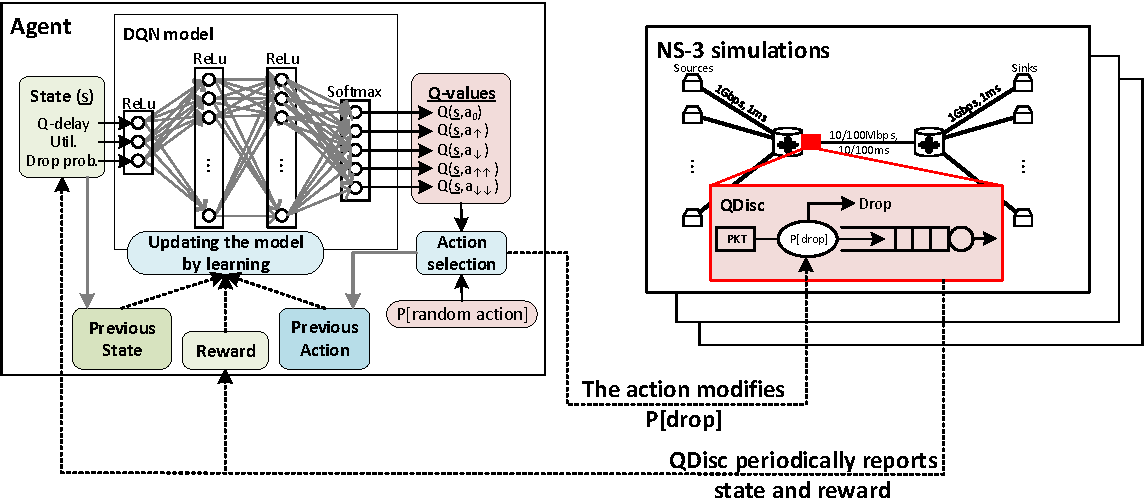
\includegraphics[width=0.9\textwidth]{Figures/rlaqm-crop.pdf}
\end{center}
\caption{RL-AQM architecture with a learning agent and NS-3 components.}
\label{fig:arch}
\end{figure*}

\begin{figure}[ht]
\begin{center}
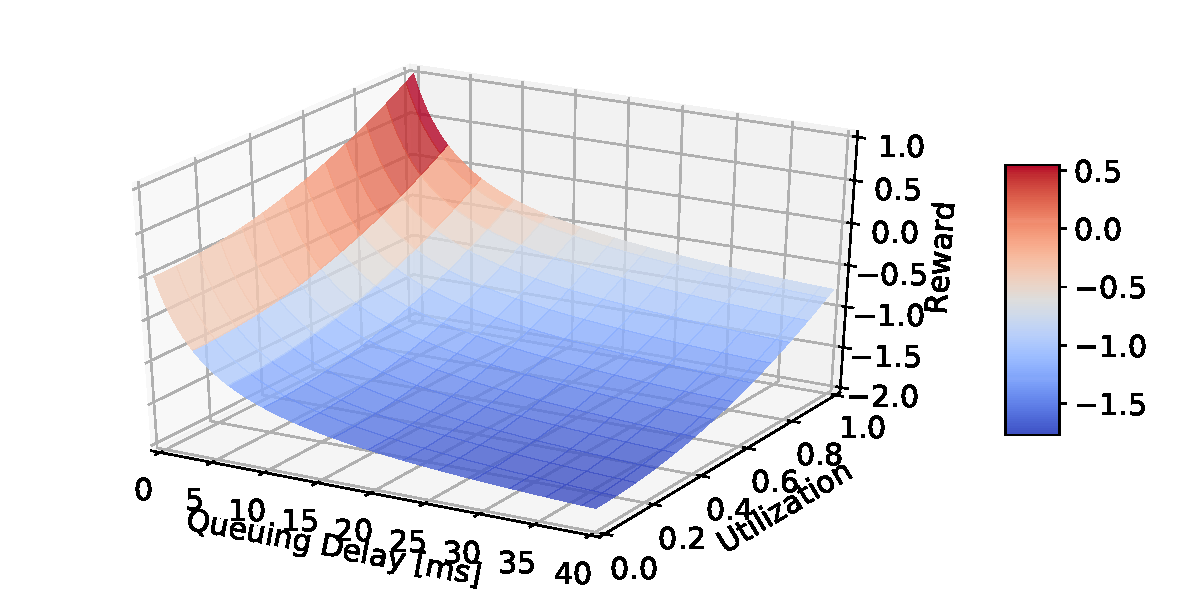
\includegraphics[width=0.45\textwidth]{Figures/reward.pdf}
\end{center}
\caption{Reward function.}
\label{fig:reward}
\end{figure}


The methods of active queue management aim at reducing queueing delay while keeping the bottleneck link fully utilized. To solve these objectives they continuously monitor both the queue and link states and make decisions on dropping or forwarding packets. Note that instead of dropping, AQMs can also mark packets with ECN Congestion Experienced (CE), reducing the number of re-transmissions in this way.
In this paper, we propose RL-AQM, an AQM algorithm that uses the tools of reinforcement learning to control the applied drop probability and thus to find a good trade-off between high link utilization and low queueing delay. The implementation of our method is based on the OpenAI Gym extension of NS-3 network simulator \cite{gawlowicz2019ns}.

According to the traditional RL approach \cite{dqn,dqnint}, the environment that represents the AQM method running inside a router can be modelled as a Markov Decision Process. The process is represented by a five-tuple $(S, A, T, R, \gamma)$ where $S$ is the state space, $A$ is the action set, $T(\underline{s}'|\underline{s},a)$ is the state transition probability where $\underline{s}',\underline{s} \in S$ and $a \in A$ , $R$ is the reward function while $\gamma \in [0,1)$ is the discount factor. In our method illustrated by Figure~\ref{fig:arch}, $\underline{s} \in S$ represents a queue state at a given point of time. $\underline{s}$ is a tuple composed of three factors: queuing delay, bottleneck link utilization and applied drop probability. We have introduced 5 actions described in Table~\ref{tab:actions} through which the applied drop probability of the AQM method can be modified with intensities. In this system model, the AQM policy is a function mapping every state to a distribution over actions: $\pi : S \longrightarrow A$. When we follow a policy $\pi$ from state $\underline{s}_t$ at time $t$, the value function can be calculated as the sum of rewards of succeeding states: $V^{\pi}(\underline{s}_t = E[ \sum^T_{i=0}\gamma^iR(\underline{s}_{t+i}, \pi(\underline{s}_t))]$. The value function ranks the policies according to the cumulative reward. The value of a single step can be calculated similarly by the Q-value function. $Q^{\pi}(\underline{s}_t,a)$ represents the expected value starting from $\underline{s}_t$, taking action $a$ and then following $\pi$. Q-value function can recursively estimated by the Bellman equation: $Q^\pi(\underline{s}_t,a) = E[R(\underline{s}_t, a) + \gamma \max_{a'}Q(\underline{s}_{t+1},a')]$. The optimal policy have the highest Q-value function over all policies. In Deep Q-Networks (DQN), the Q-value function is approximated by a neural network and the reinforcement learning process uses the previously introduced Bellman equation.

The architecture of the proposed method is depicted in Figure~\ref{fig:arch}. It consists of two components: 1) the OpenAI-based learning agent, and 2) the NS3 simulation environment. The NS-3 environment implements the simulation scenarios using a dumb-bell topology with various traffic intensities and link properties (bandwidth and RTT), and the frame of the proposed RL-AQM method as a queuing discipline (QDisc in NS-3 terminology) that simple drops packets at arrival with a specific probability, maintains state information and evaluates the reward function. The business logic is fully implemented by the Agent. The simulator is connected to the Agent and reports the current state of the QDisc (queueing delay, utilization and actual drop probability) periodically, in every 20~ms in our setting. It also computes the reward ($R(\underline{s}_t,a_t)$) for the simulation period elapsed since the last update of drop probability (using action $a_t$ at time $t$). The Agent takes the computed reward and the new state $\underline{s}_{t+1}$, and applies the Bellman equation to update the DQN model. Then the new state $\underline{s}_{t+1}$ is fed into the DQN to calculate the Q-values $Q(\underline{s}_{t+1},a)$ for each action $a$. The candidate action to be performed is the one with the highest Q-value: $a_{t+1} = \arg_a\max Q(\underline{s}_{t+1},a)$. To determine the action to be executed we also apply further heuristics and random selection. 

\begin{table}[ht]
\centering
%\begin{center}
\label{tab:actions}
\caption{Possible actions}
\begin{tabular}{ | m{2em} | m{14em} |  }
\hline
$a_{0}$  & do not modify the drop probability \\ 
\hline
$a_{\uparrow}$ & increase drop probability by 0.01 \\ 
\hline
$a_{\downarrow}$ & decrease drop probability by 0.01 \\
\hline
$a_{\uparrow\uparrow}$ & increase drop probability by 0.1 \\
\hline
$a_{\downarrow\downarrow}$ & decrease drop probability by 0.1 \\
\hline
\end{tabular}
%\end{center}
\end {table}


\subsection{Action selection}
Packets arrive in bursts at the bottleneck and thus they result in temporal loads that are handled by the AQM methods. However, between two such bursts the link is not overloaded and the queue is almost always empty. When we first applied RL-AQM, it showed a very slow convergence since the DQN also learned Q-values for the trivial cases. To fasten learning process, we introduced two simple heuristics: 1) if the queueing delay is less than 1~ms and the drop probability is 0, we select $a_0$ and keep drop probability at zero, 2) if the queueing delay is less than 1~ms and the drop probability is not zero, we select $a_\downarrow\downarrow$ that reduces the drop probability by $0.1$. In addition to these trivial cases, we also allow the model to discover new decisions by giving some probability to choose a random action to be executed. This enables the model to continuously learn and adapt to the changes in the environment. After the pre-training phase, this probability was set to $0.01$ in our setting.

\subsection{Pre-training}
At the beginning the Agent's internal model is empty, it basically knows nothing about the environment and the optimal policy $\pi$. To learn the appropriate policy and its Q-value function, we show example episodes to the Agent during the pre-training phase. The method is the same as in Figure~\ref{fig:arch} with a single exception: the probability of random action selection is not constant. It starts with $0.9$ in the first episode and decays exponentially with a minimum of $0.01$. Accordingly, in the $i$th episode it is set to $\max(0.9^i, 0.01)$. Each pre-training episode covers a 120 sec long simulation with 9 sections with various traffic intensities (see Figure~\ref{fig:numflows}). The bottleneck capacity and the link delays are fixed and a dumb bell topology is used.

\begin{figure}[t]
\begin{center}
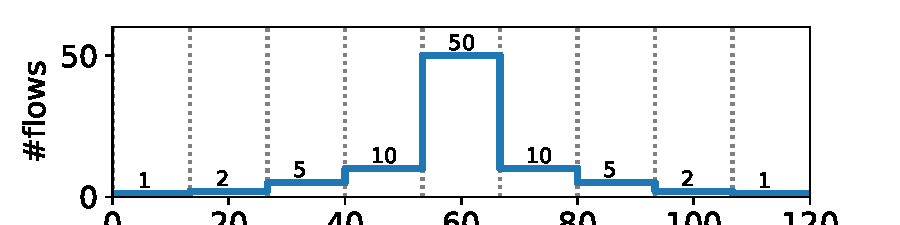
\includegraphics[width=0.45\textwidth]{Figures/flownum.pdf}
\end{center}
\caption{The simulation is split into 9 sections with various traffic intensities.}
\label{fig:numflows}
\end{figure}


\subsection{Reward function}
The core essence of reinforcement learning methods is the good choice of reward function. The reward is the optimization objective used for finding the optimal policy $\pi$. In contrast to traditional methods like PIE AQM or CoDel where a target queueing delay parameter is needed, we have decided to follow the idea of \cite{steeringgsp}. This paper shows that there is no unified target delay that is optimal in all cases. The good target value also depends on the number of flows in the system. For example, large number of flows can fully utilize the link with smaller target delays. This idea led us to define a reward function depicted in Figure~\ref{fig:reward} that takes both the utilization and queuing delay into account: $R(U,D) = (U^2-0.5)+(\frac{2}{1+D}-1.5)$ where $U \in [0,1]$ is the link utilization and $D \ge 0$ is the queueing delay in ms. One can observe that reward function returns values from the range $(-2,1]$. Our goal is to find a good trade-off between low delay and good link utilization.


\section{Evaluation}
The network topology used in this work to evaluate the proposed RL-AQM method is shown in Figure~\ref{fig:arch}. It consists of 50 source and 50 sink nodes. They share the same bottleneck between n0 and n1. Link capacities between the sources and n0, and the sinks and n1 are set to be 1~Gbps. The bottleneck link between n0 and n1 is set to 10~Mbps or 100~Mbps, depending on the scenario. The end-to-end RTT between sources and sinks are varied between 20 and 100~ms.
In every scenario, the simulation time is 120 seconds that is split into 9 sections with various number of flows (see Figure~\ref{fig:numflows}). Each flow is a TCP connection with NewReno congestion control working in non-ECT mode. If it is not mentioned otherwise, we present the results of pre-trained Agents (with 200 pre-training episodes).

%\begin{figure}[t]
%\begin{center}
%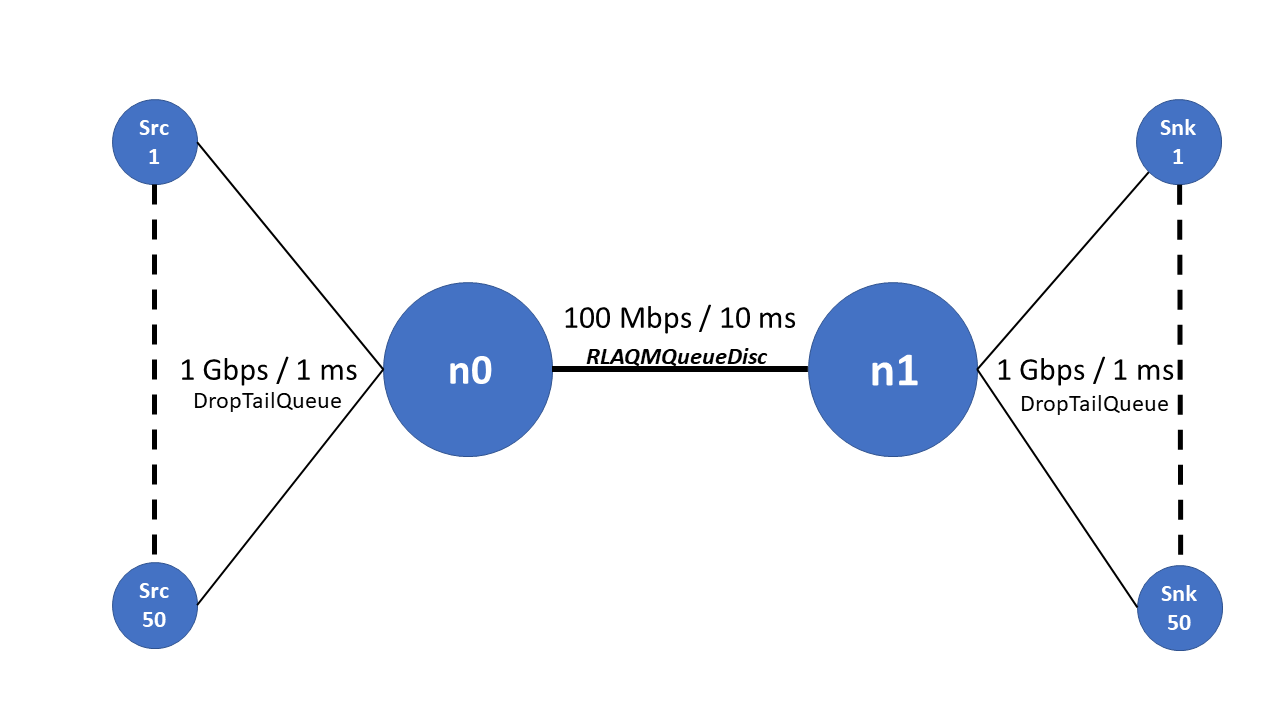
\includegraphics[width=0.45\textwidth]{Figures/ch4topo.png}
%\end{center}
%\caption{Network topology.}
%\label{fig:topo}
%\end{figure}

\subsection{Pre-training and convergence}
Figure~\ref{fig:reward_delay} shows the convergence of the average reward (blue curve) and queueing delay (red dashed curve) over the pre-training episodes. Note that the maximum value of the applied reward function is $1.0$. Episode~1 starts with an empty internal model.  One can see that after the first 10 episodes we reach $0.82$ and then the reward stabilizes around this point. The queuing delay is near 50~ms in Episode~1 and it reaches 20~ms by the end of pre-training. Some outlier episodes can also be seen but in these cases the probability of random action selection was still high, resulting in small drop ratio in the QDisc that led to larger queueing delays, implicating the lower reward value.

\begin{figure}[b]
\begin{center}
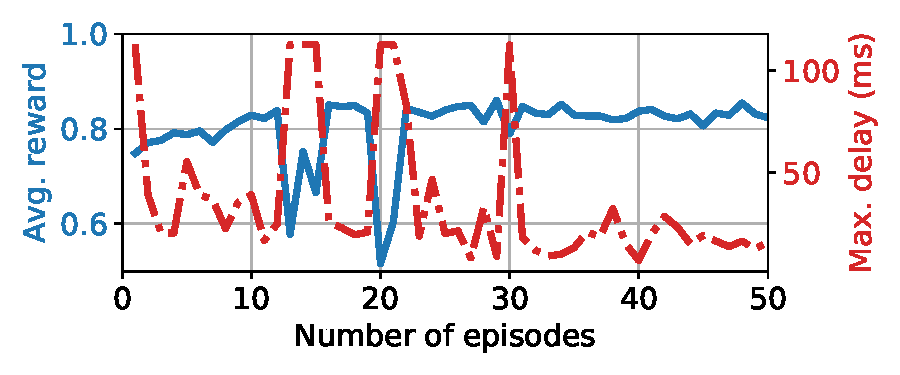
\includegraphics[width=0.45\textwidth]{Figures/reward_delay.pdf}
\end{center}
\caption{Rewards and observed maximum delays over the episodes}
\label{fig:reward_delay}
\end{figure}

As mentioned previously, the Agent can also apply an action selected randomly. During the pre-training phase, the probability of random selection is high which enables the agent to trial various actions and learn their effects.  The probability of this decision is decreasing in every pre-training episode. Figure~\ref{fig:reward_epsolon} shows the same reward (blue) as the previous figure and the probability of random action selection (red). When this probability is high, the less stable agent behaviour may lead to episodes with low reward (e.g., Episode 12 and 20), but it is natural in the pre-training period. 
%We can see in episode 12 the Agent chose random action because the probability of it is over 0.3. The event is similar at episode 20. In this episode, the probability is 0.15. 

\begin{figure}[b]
\begin{center}
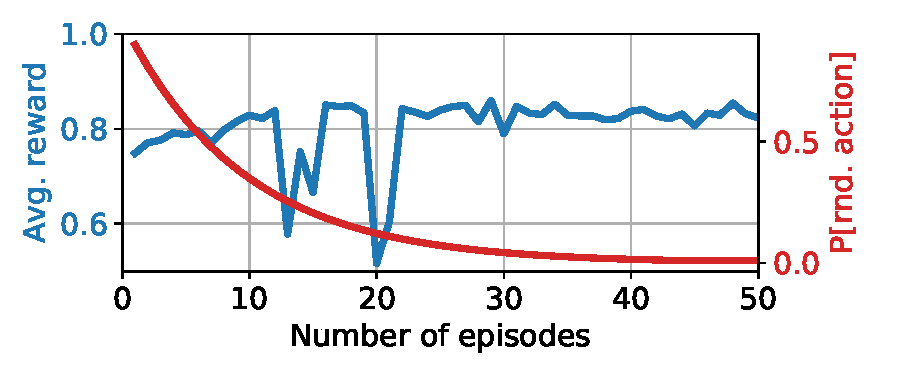
\includegraphics[width=0.45\textwidth]{Figures/reward_epsilon.pdf}
\end{center}
\caption{Rewards and the probability of random action selections over episodes}
\label{fig:reward_epsolon}
\end{figure}

\subsection{Comparison to PIE AQM}
In order to consolidate the proposed RL-AQM, we will compare its performance to PIE AQM \cite{pan2017proportional} under the same network topology. We have selected PIE among the others AQMs because PIE is also based on control theory to oversee queue size and modify drop  probability accordingly, as in the proposed RL-AQM. PIE uses PI controller to update the drop probability whereas the proposed AQM relies on the DQN-based Agent. Figure~\ref{fig:rl10mbps20ms} shows the total throughput on the bottleneck link (top), the per-flow throughput curves (middle), and the queue delay (bottom) under the action of RL-AQM when the bottleneck link is set to 10~Mbps and RTT is 20~ms. Figure~ \ref{fig:pie10mbps20ms} depicts these three graphs for PIE AQM. One can observe that in comparison to PIE, RL-AQM significantly reduces the queue delay and results in the same link utilization. RL-AQM managed to keep the average queue delay almost all the time under the PIE's delay target value (15~ms as default) especially when the number of flows is high (50-60 secs). Even when the number of flows decreases after the 80th second, PIE can not quickly push the delay under the target value because it gradually decreases the drop probability value according to its algorithm. Both AQMs obtain the same throughput value and the fairness of flows are also relatively the same.  
%The control system in PIE consists of three main parts:  a) random dropping at enqueuing as our proposed AQM. When a packet arrives, a random decision is made about dropping the packet or not based on a drop probability. PIE skips the random drop if the queue delay is smaller than half of the Target delay (QDELAY\_REF =15 milliseconds) , b) periodic drop probability updates, PIE uses the Proportional Integral (PI) controller method to update the drop probability based on the current queue delay and whether the delay is trending up or down. The drop probability in PIE is calculated based on the following equation 
%\begin{equation}
%\resizebox{.9\hsize}{!} {p = \alpha * (current\_qdelay -QDELAY\_REF) +  \beta * (current\_qdelay - PIE-> qdelay\_old)}
%\end{equation}
%and then p decreased if it is in the range (0.1-0.000001). Otherwise, the new drop probability equal:
%\begin{equation}
%    drop probability = drop probability + p
%\end{equation}
%$\alpha (default 0.125)$ and $\beta (default 1.25)$ are controller parameters. In the proposed AQM the drop probability is calculate by the agent. The third component  c) latency calculation is obtained in PIE using one of two ways: 1) using little's law or 2) using other techniques, e.g, Time-Stamp the packets at enqueue. Whereas in the proposed AQM, queue length is used to obtain the queue delay(latency).     
\begin{figure}[t]
\begin{center}
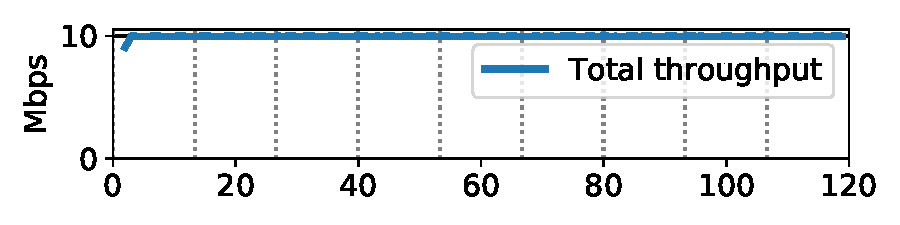
\includegraphics[width=0.45\textwidth]{Figures/rl_10mbps_10ms_total.pdf} \\
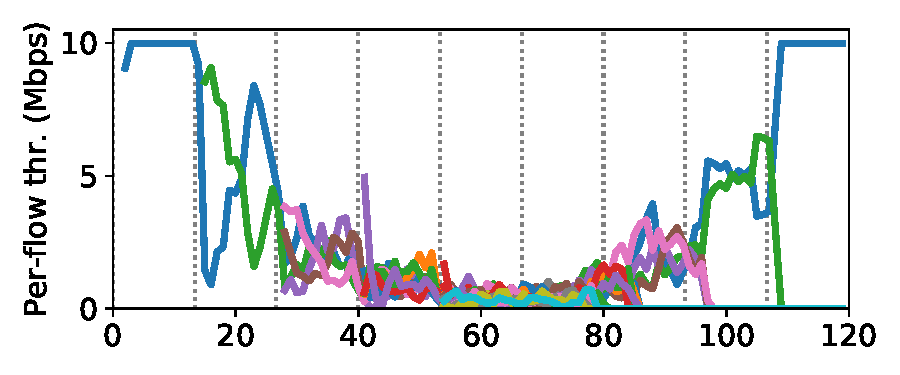
\includegraphics[width=0.45\textwidth]{Figures/rl_10mbps_10ms_flow.pdf} \\
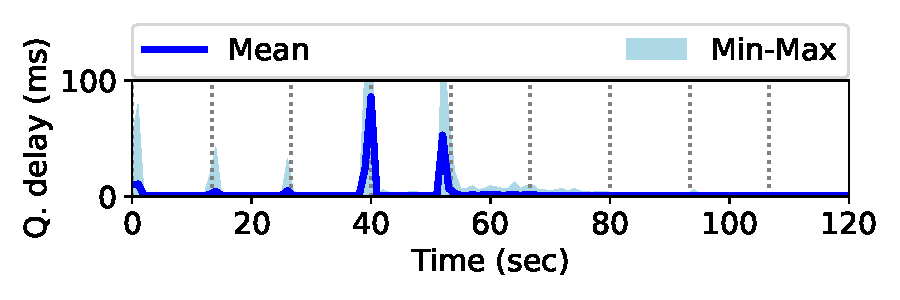
\includegraphics[width=0.45\textwidth]{Figures/rl_10mbps_10ms_delay.pdf}
\end{center}
\caption{RL-AQM, BN capacity=10~Mbps RTT=20~ms}
\label{fig:rl10mbps20ms}
\end{figure}

\begin{figure}[t]
\begin{center}
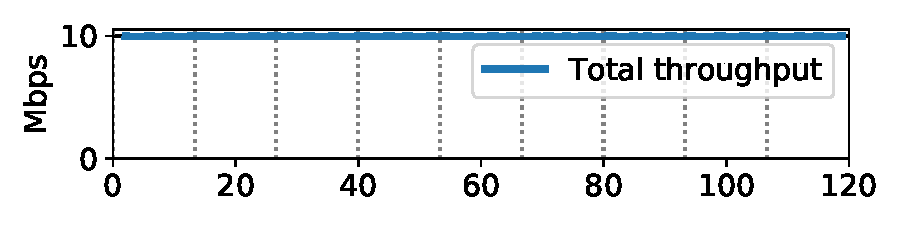
\includegraphics[width=0.45\textwidth]{Figures/pie_10mbps_10ms_total.pdf} \\
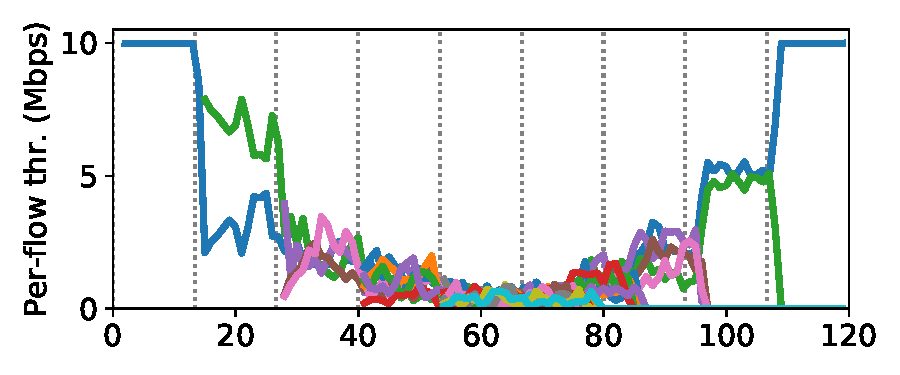
\includegraphics[width=0.45\textwidth]{Figures/pie_10mbps_10ms_flow.pdf} \\
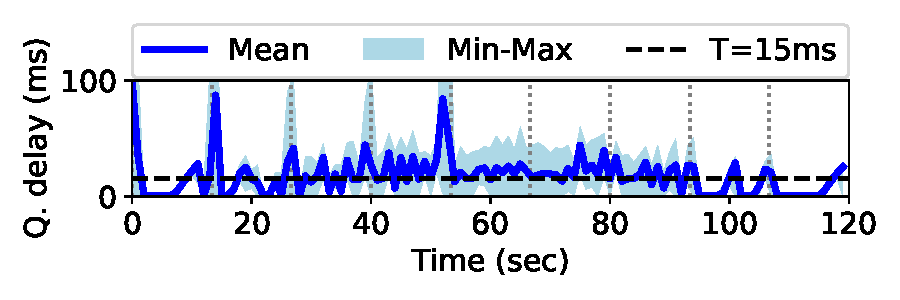
\includegraphics[width=0.45\textwidth]{Figures/pie_10mbps_10ms_delay.pdf}
\end{center}
\caption{PIE AQM, BN capacity=10~Mbps, RTT=20~ms}
\label{fig:pie10mbps20ms}
\end{figure}
Figure~\ref{fig:rl100mbps20ms}-\ref{fig:pie100mbps20ms} show the same three metrics after we increased the bottleneck link capacity to 100~Mbps. PIE shows better performance in the average queue delay comparing to its performance under the 10~Mbps but still higher than the PIE's target value. RL-AQM has managed to keep the average queueing delay low in most of the simulation time. It generates congestion signals earlier than PIE, leading to that TCP sources starts reducing their sending rates without waiting the queue to get full. % and then starts to drop/drain the queue. 
On the other side, the utilization seen for RL-AQM is slightly worst than for PIE, it is the price we have to pay for the low delay. However, one can also observe that large deviations can only be seen when the number of flows are 1 or 2. In other cases, the total throughput is almost 100~Mbps all the time. In contrast to PIE, RL-AQM reward function was designed to find a good trade-off between the utilization and delay, and do not contain any target value. The reward can be increased by decreasing the delay at the expanse of utilization for some level, and vice-versa. Note that this behavior is similar to what a virtual queue does with a slightly smaller serving rate than the one of associated physical queue.
%RL-AQM drops one packet before the queue delay getting high as calculated by the reward function and as a consequence when the Agent decides regardless the queue delay.
\begin{figure}[ht]
\begin{center}
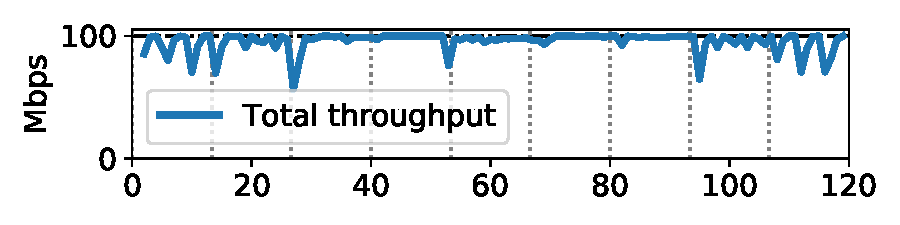
\includegraphics[width=0.45\textwidth]{Figures/rl_100mbps_10ms_total.pdf} \\
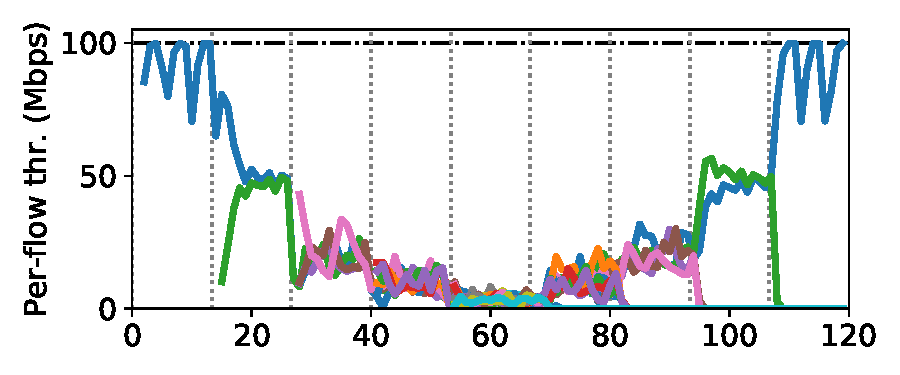
\includegraphics[width=0.45\textwidth]{Figures/rl_100mbps_10ms_flow.pdf} \\
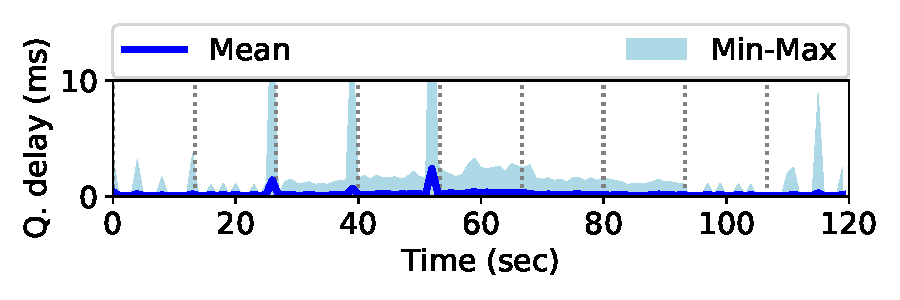
\includegraphics[width=0.45\textwidth]{Figures/rl_100mbps_10ms_delay.pdf}
\end{center}
\caption{RL-AQM, BN capacity=100~Mbps, RTT=20~ms}
\label{fig:rl100mbps20ms}
\end{figure}

\begin{figure}[ht]
\begin{center}
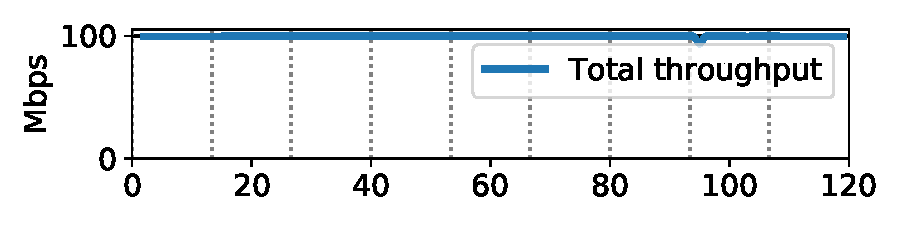
\includegraphics[width=0.45\textwidth]{Figures/pie_100mbps_10ms_total.pdf} \\
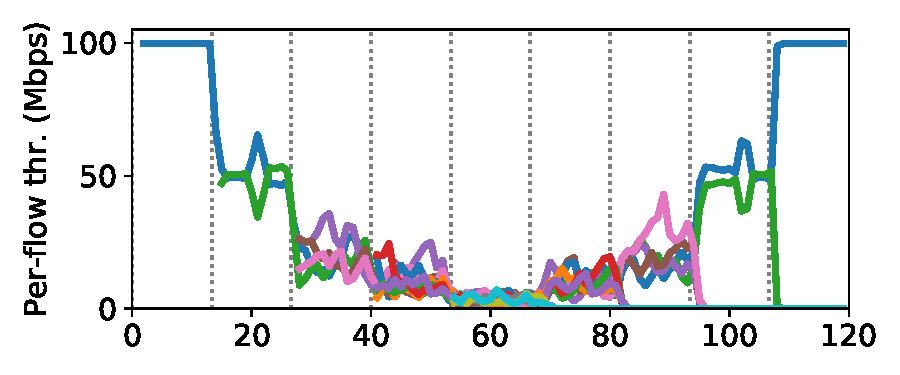
\includegraphics[width=0.45\textwidth]{Figures/pie_100mbps_10ms_flow.pdf} \\
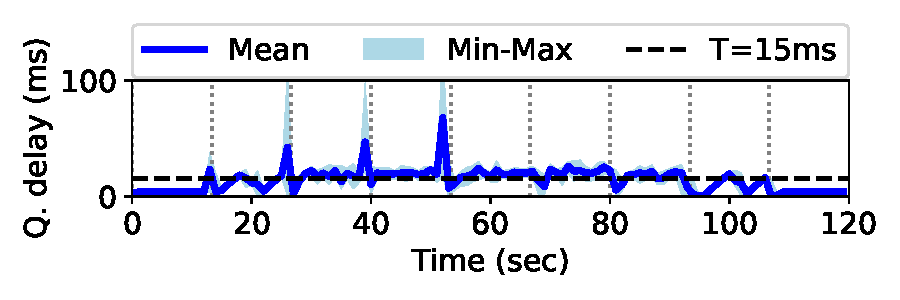
\includegraphics[width=0.45\textwidth]{Figures/pie_100mbps_10ms_delay.pdf}
\end{center}
\caption{PIE AQM, BN capacity=100~Mbps, RTT=20~ms}
\label{fig:pie100mbps20ms}
\end{figure}

\subsection{Generalization}
During the pre-training phase, we fix the parameters of the simulations. Though the number of flows are varied in a wide range, the bottleneck capacity and the RTT remain the same over the pre-training episodes. To check the generalization ability of a pre-trained Agent, we have executed simulations with different bottleneck capacity and RTT. 
We created an Agent trained with the following parameters:  bottleneck capacity was 10~Mbps and the RTT was 20~ms. We used this Agent in evaluations with different settings. Figure~\ref{fig:rl_tr10_100mbps20ms} shows the first case when the bottleneck capacity is 100~Mbps instead of 10~Mbps while the RTT is still 20~ms. One can see that the total throughput of flows reaches the maximum capacity and flows share the bottleneck in a fair way. However, the time needed for reacting to temporal bursts is longer than it is in Figure~\ref{fig:rl100mbps20ms}, esp. when the number of flows is 1 or 2. Note that it is also reflected by the higher queueing delays in these simulation sections. The reason is that the model has been trained with lower bandwidth where the decision is based on fewer packets, so the congestion signal (drop probability) generated by the AQM is higher than what is actually required for reducing the delay.
%In this case, more packets come and the model has to adapt to it.


\begin{figure}[t]
\begin{center}
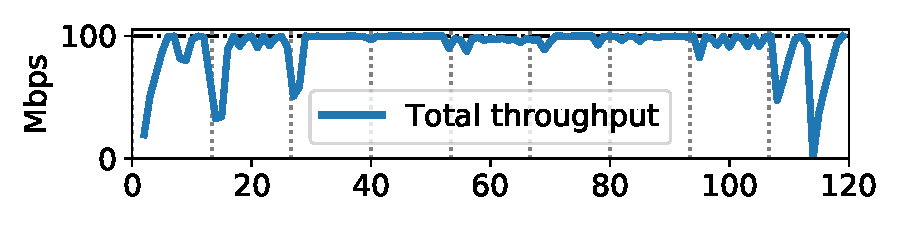
\includegraphics[width=0.45\textwidth]{Figures/rl_tr10mbps-100mbps_10ms_total.pdf} \\
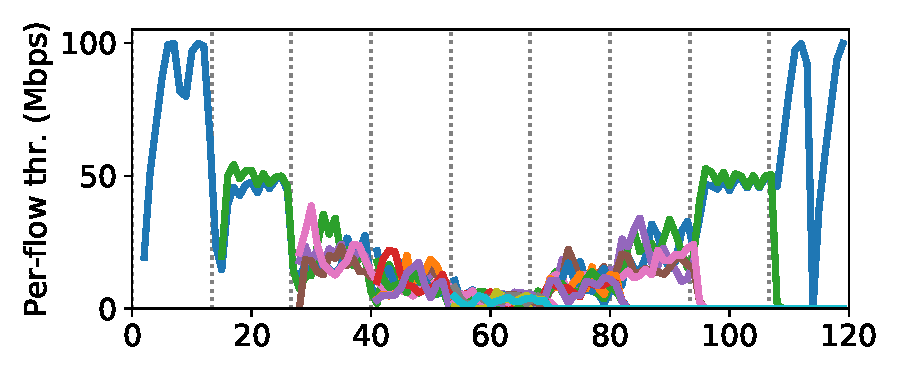
\includegraphics[width=0.45\textwidth]{Figures/rl_tr10mbps-100mbps_10ms_flow.pdf} \\
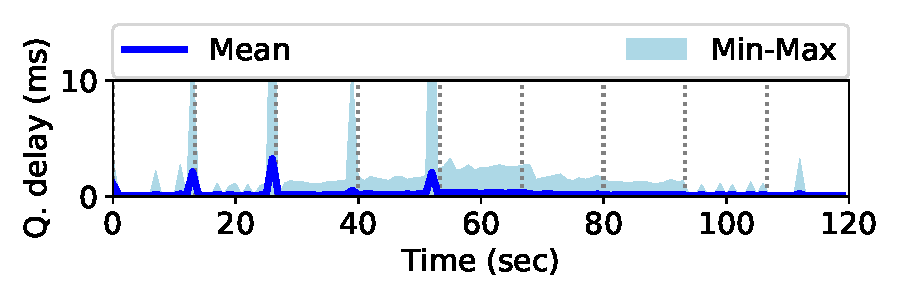
\includegraphics[width=0.45\textwidth]{Figures/rl_tr10mbps-100mbps_10ms_delay.pdf}
\end{center}
\caption{Generalization ability of RL-AQM, BN cap. increased to 100Mbps}
\label{fig:rl_tr10_100mbps20ms}
\end{figure}

Figure~\ref{fig:rl_tr10_10mbps100ms} depicts the second case where the bottleneck capacity remains 10~Mbps, but the RTT is 100~ms instead of 20~ms. Despite the feedback loop of TCP's congestion control is much longer, the pre-trained Agent results in almost perfect utilization and good fairness among flows. The large RTT results in longer ramp-up in the sending rates. The longer queueing delays are natural results of the longer RTT, since TCP is RTT-clocked. RL-AQM changes the drop probability, but flows do not react until 100~ms. When the number of flows is high, high average queueing delays can be observed. It is the same situation: the AQM makes changes, but flows needs 100~ms for reaction.

\begin{figure}[t]
\begin{center}
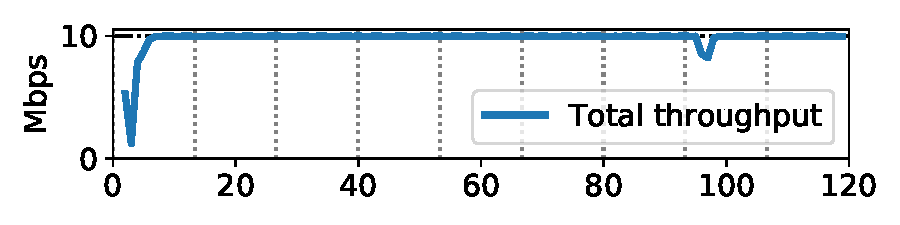
\includegraphics[width=0.45\textwidth]{Figures/rl_tr10mbps-10mbps_100ms_total.pdf} \\
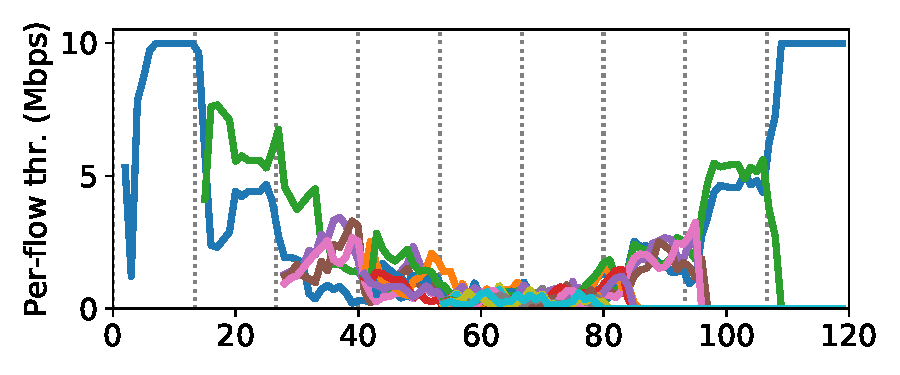
\includegraphics[width=0.45\textwidth]{Figures/rl_tr10mbps-10mbps_100ms_flow.pdf} \\
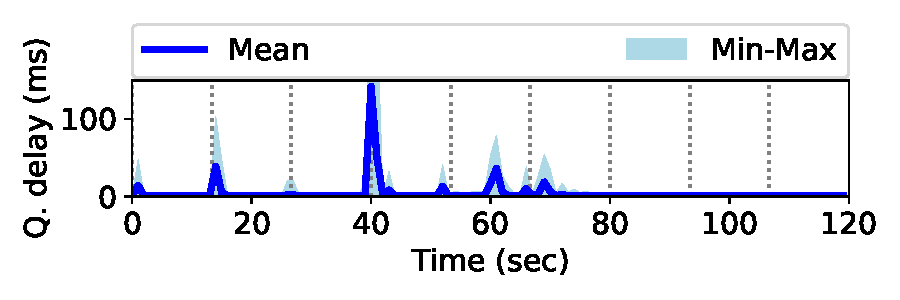
\includegraphics[width=0.45\textwidth]{Figures/rl_tr10mbps-10mbps_100ms_delay.pdf}
\end{center}
\caption{Generalization ability of RL-AQM, RTT increased to 100ms}
\label{fig:rl_tr10_10mbps100ms}
\end{figure}

%In general, we can see the model can be used in different scenarios and can reach high throughput and a low queueing delay. 

%\section{Open-AI ns3-gym for Network Qdisc}
%The agent in the machine learning is learning how to make best out in the given environment, the environments offers an options (Observation state) and reward at a time and the agent keeps doing experiments based on trying different actions in the aim to get higher reward.  OpenAI Gym is tool that provides a space for the agents to predict the behavior of the corresponding environment, this tool is  combined with the ns3 to provide a framework known as ns3-gym in order to encourage usage of RL in networking research \cite{gawlowicz2019ns}.  The general figure of the RL is re-involved in figure 1, in our work we have designed new qdisc to be able to get the queue delay directory during running time as an observation state, in another words, in each time-step (or tick) the current queue delay is provided to the agent along with a reward.
%
%We have followed the same workflow that has been introduced in \cite{gawlowicz2019ns},  the network topology is shown in figure 2, The designed queue disc (ns3::RLAqmQueueDisc) is connected to the gym environment as in figure 3.


%the simulation time in 120 seconds and the number of tcp flows is 100. The action space is shown in Table 1, the agent decides witch action number between (0-4) will be executed based on the state of the observation space. Every 0.1 second, the environment (the ns3 topology) is set to provide the agent with the current state through the observation space with is represented in this work by four factors; the queue delay, the utilization, the drop probability and the reward. These four factors had been implemented in the proposed ns3 queue disc under the name (rlaqm-queue-disc). 



%Figure 4, shows the GetObservation implentation in the gym environment and it also illustrates how the box is filled with the current queue delay, the utilization and the drop probability functions, the initial values for the three factors are also showed. 
% ==== Fig 4


% on the current queue delay and the reward, the agent sends back the action to be executed. In this work, the agent  sets the drop probability of the queue disc by the SetDropProb() function which is also implemented inside our qdisc (ns3::RLv1QueueDisc), the ExecuteActions callback of this work is shown in figure 5. \color{red} More here about the drop is needed\color{black}. 
%The agent  sets the drop probability of the queue disc by the SetDropProb() function which is also implemented inside our qdisc, the ExecuteActions callback of this work is shown in figure 5. Our queue disc implementation drops the incoming packets based on two facts; 1) if the queue is full (as default), 2) if the packet arrives and drop probability in the queue is above 1.0.  

%The utilization is calculated based on the following equation ``\eqref{eq4}'': 
%\begin{equation}
%{\textstyle Utilization = clip (\frac {dequeue rate} {MIN (Enqueu rate, BNC)} , 0 , +1) }\label{eq4}
%\end{equation}
%Where BNC is the bottleneck link capacity. To avoid the offshoot of the utilization function, we clip it to be between 0 and 1. 
%The reward function is calculated based on ``\eqref{eq5}'': 
%\begin{equation}
%Reward =  0.5 * utilization +\frac{ 0.3 } {1.0 + QD} + 0.2(1-DP)\label{eq5}
%\end{equation}
%where QD and DP are the current queue delay and the drop probability respectively. The agent is implemented by python. Table 3 shows the properties of the agent. We separated the process of the agent into two steps. first, to train the agent and obtain the best model and save it in a model file.The best model is represented by the episode which has the highest number of rewards. Figure 6 illustrates the rewards sum if each episode in this work.  Second, we use the best model file as a learned agent to interact with the ns3 topology environment. The agent is set to train the network using the 4 layers model free Deep queue learning (DQN). figure 7 shows how the agent implemented to train the neural network by two layers each with 16 neurons.   

%\begin{table}[ht]
%\centering
%\begin{center}
%\caption{\label{tab:table-name} The Agent characteristic .}
%\begin{tabular}{ | m{14em} | m{2em} |  } 
%\hline
%Total number of episodes  & 20 \\ 
%\hline
%Max steps in each episode  & 100 \\ 
%\hline
%the exploration rate (epsilon) & 0.9 \\
%\hline
%epsilon\_min & 0.01 \\
%\hline
%epsilon\_decay & 0.999 \\
%\hline
%Actions (cwSize) & 5 \\
%\hline
%\end{tabular}
%\end{center}
%\end {table}



%\section{How the System Works}
%To train the agent, a python file is set to run the simulation with 100 episode. Each episode form the training process is designed to generate a figure,under the log directory, which contains 4 sub-figures; the Queue delay, the utilization, the drop probability of the queue and the reward (over 6000 steps) respectively. Each 1 sec from the simulation time represents 50 steps in the agent. the time of any step can be calculated by multiply the step by 120 over 6000 ie (step 4800 = 96 sec). figure 8 shows the sub-figures of the best episode which has the highest rewards value. After training the model, the episode with the best results is saved to be used as a best model to avoid consuming resources and time of training the network each time we run the simulation. Another python file is set to run the simulation with the best trained episode directly. After executing  the best model, the throughput in bottleneck link will be generated in a form of curve over time as shown in figure (). To be more accurate we obtained the throughput using the FlowMonitor in Ns3 by filtering only the flows (from source to distention) and ignore the feedback and overhead flows, the filtered flows are saved in .csv file. However, the pcap file is also generated if other statistics are needed.
%The simulation topoloyg and network parameters can be changed as any ns3 simulation and the queue disc from ns3 library can also be used like normal ns3 topology, the RLAQM-queue-disc is only included inside the ns3-gym library.(link to github) 
% ==== Fig 8

\section{Conclusion}
This paper proposes RL-AQM, a new AQM method based on reinforcement learning to manage the network resources and keep the queue delay low at the same time. The proposed method has the advantage that it adapts to the changing network environment automatically, without the need of extra parameters and parameter tuning. The queue delay control is done by an Agent implementing a Deep Q-learning model. We implemented the RL-AQM in NS-3 network simulator with the use of OpenAI Gym tools. Our evaluation results demonstrate that RL-AQM provides good performance in different types of networks (different bottleneck link capacities and RTTs). For the purpose of validation, we have compared its performance to the state-of-the-art PIE AQM. PIE is based on control theory (PI) with several parameters. 
%However, The compassion is done based on throughput and queue delay values under varied number of TCP flows. RL-AQM outperforms PIE.  
The evaluation results show that RL-AQM can keep the queue delay under PIE's target delay  (15~ms) during most of the simulation time. The price of ultra-low delay is that some bandwidth is sacrificed, esp. if the number of flows is small, leading to a virtual queue-like behavior.
%The simple mechanisms of the applied queueing discipline and the agent-based control fit well to the concept of programmable data planes, where the methodthe implementation of the proposed AQM using the future network programming language (P4) and checking its performance under SDN since it's based on RL and parameterless. 



%\section*{Acknowledgment}
%Application Domain Specific Highly Reliable IT Solutions” project  has been implemented with the support provided from the National Research, Development and Innovation Fund of Hungary, financed under the Thematic Excellence Programme TKP2020-NKA-06 (National Challenges Subprogramme) funding scheme.
%Supported by the ÚNKP-20-4 New National Excellence Program of the Ministry for Innovation and Technology from the source of the National Research, Development and Innovation Fund.
%The research has partially been supported by the European Union, co-financed by the European Social Fund (EFOP-3.6.2-16-2017-00013, Thematic Fundamental Research Collaborations Grounding Innovation in Informatics and Infocommunications).



\bibliographystyle{./bibliography/IEEEtran}
\bibliography{./bibliography/IEEEabrv,./bibliography/IEEEexample}




\end{document}
